\documentclass[BCOR1cm, twoside, openright, titlepage, bibtotoc, abstracton]{scrartcl}

\usepackage[german,english]{babel}
\usepackage[T1]{fontenc}
\usepackage[utf8]{inputenc}
\usepackage{amsmath,amstext,amssymb}
\usepackage{geometry}
\usepackage{lmodern}
\usepackage{titlesec}
\usepackage[a4paper,pagebackref,hyperindex=true]{hyperref}
\usepackage{caption}
\usepackage{subfigure}
\usepackage{booktabs}
\usepackage{pdfpages}
\usepackage{appendix}
\usepackage{minitoc}
\usepackage{algorithm}

\usepackage{algorithmic}
\renewcommand{\algorithmicrequire}{\textbf{Input:}}
\renewcommand{\algorithmicensure}{\textbf{Output:}}

\usepackage[scaled=0.8]{beramono}

\usepackage{fancyhdr}                   
\setlength{\headheight}{25.2232pt}

\selectlanguage{english}

% listings
\usepackage{listings}
\lstset{ %
  language=C++, % choose the language of the code
  basicstyle=\small\ttfamily, % the size of the fonts that are used for the code
  numbers=left, % where to put the line-numbers
  numberstyle=\small\ttfamily\color[rgb]{0.6,0.6,0.6}, % the size of the fonts that are used for the line-numbers
  stepnumber=1, % the step between two line-numbers. If it's 1 each line
  xleftmargin=4mm,
  % will be numbered
  numbersep=5pt, % how far the line-numbers are from the code
  backgroundcolor=\color{white}, % choose the background color. You must add \usepackage{color}
  showspaces=false, % show spaces adding particular underscores
  showstringspaces=false, % underline spaces within strings
  showtabs=false, % show tabs within strings adding particular underscores
  %frame=l, % adds a frame around the code
  frame=single,
  tabsize=4, % sets default tabsize to 2 spaces
  breaklines=true, % sets automatic line breaking
  breakatwhitespace=false, % sets if automatic breaks should only happen at whitespace
  % also try caption instead of title
  escapeinside={@}{@}, % if you want to add a comment within your code
  morekeywords={*,...,omp, parallel,__local,__global,__kernel,value_type}, % if you want to add more keywords to the set
  keywordstyle=\color[rgb]{0,0,1},
  commentstyle=\color[rgb]{0.133,0.545,0.133}\textit,
  stringstyle=\color[rgb]{0.627,0.126,0.941},
}
\newcommand{\matlab}[2] {\vspace{3mm}\lstinputlisting[title={#2}]{#1}}

% Links in pdf
\usepackage{color}
\newcommand{\blue}{ \color{blue} }
\definecolor{linkcol}{rgb}{0,0,0.4}
\definecolor{citecol}{rgb}{0.5,0,0}

\hypersetup
{
bookmarksopen=true,
pdftitle="Master Thesis",
pdfauthor="Max Muster",
pdfsubject="Title of the Document", %subject of the document
%pdftoolbar=false, % toolbar hidden
pdfmenubar=true, %menubar shown
pdfhighlight=/O, %effect of clicking on a link
colorlinks=true, %couleurs sur les liens hypertextes
pdfpagemode=None, %aucun mode de page
pdfpagelayout=SinglePage, %ouverture en simple page
pdffitwindow=true, %pages ouvertes entierement dans toute la fenetre
linkcolor=linkcol, %couleur des liens hypertextes internes
citecolor=citecol, %couleur des liens pour les citations
urlcolor=linkcol %couleur des liens pour les url
}

% nicer backref links
\renewcommand*{\backref}[1]{}
\renewcommand*{\backrefalt}[4]{%
\ifcase #1 %
(Not cited.)%
\or
(Cited on page~#2.)%
\else
(Cited on pages~#2.)%
\fi}
\renewcommand*{\backrefsep}{, }
\renewcommand*{\backreftwosep}{ and~}
\renewcommand*{\backreflastsep}{ and~}


\newcommand{\ve}[1]{
	\mathbf{#1}
	%\vec{#1}
}

\newcommand{\grad}{ \textbf{\,grad\,} }
\providecommand{\argmin}{\operatorname*{argmin}} % operatorname makes _{..} appear centered
\newcommand{\dx}{ \,\ve{dx} }

\renewcommand{\a}{\ve{a}}
\renewcommand{\b}{\ve{b}}
\renewcommand{\c}{\ve{c}}
\renewcommand{\d}{\ve{d}}
\newcommand{\e}{\ve{e}}
\newcommand{\f}{\ve{f}}
\newcommand{\g}{\ve{g}}
\newcommand{\h}{\ve{h}}
\renewcommand{\i}{\ve{i}}
\renewcommand{\j}{\ve{j}}
\renewcommand{\k}{\ve{k}}
\renewcommand{\l}{\ve{l}}
\newcommand{\m}{\ve{m}}
\newcommand{\n}{\ve{n}}
\renewcommand{\o}{\ve{o}}
\newcommand{\p}{\ve{p}}
\newcommand{\q}{\ve{q}}
\renewcommand{\r}{\ve{r}}
\newcommand{\s}{\ve{s}}
\renewcommand{\t}{\ve{t}}
\renewcommand{\u}{\ve{u}}
\renewcommand{\v}{\ve{v}}
\newcommand{\w}{\ve{w}}
\newcommand{\x}{\ve{x}}
\newcommand{\y}{\ve{y}}
\newcommand{\z}{\ve{z}}

\newcommand{\A}{\ve{A}}
\newcommand{\B}{\ve{B}}
\newcommand{\C}{\ve{C}}
\newcommand{\D}{\ve{D}}
\newcommand{\E}{\ve{E}}
\newcommand{\F}{\ve{F}}
\newcommand{\G}{\ve{G}}
\renewcommand{\H}{\ve{H}}
\newcommand{\I}{\ve{I}}
\newcommand{\J}{\ve{J}}
\newcommand{\K}{\ve{K}}
\renewcommand{\L}{\ve{L}}
\newcommand{\M}{\ve{M}}
\newcommand{\N}{\ve{N}}
\renewcommand{\O}{\ve{O}}
\renewcommand{\P}{\ve{P}}
\newcommand{\Q}{\ve{Q}}
\newcommand{\R}{\ve{R}}
\renewcommand{\S}{\ve{S}}
\newcommand{\T}{\ve{T}}
\newcommand{\U}{\ve{U}}
\newcommand{\V}{\ve{V}}
\newcommand{\W}{\ve{W}}
\newcommand{\X}{\ve{X}}
\newcommand{\Y}{\ve{Y}}
\newcommand{\Z}{\ve{Z}}

\hyphenation{inter-grid}

\newenvironment{packed_item}{
\vspace{-2mm}
\begin{itemize}
  \setlength{\itemsep}{1pt}
  \setlength{\parskip}{0pt}
  \setlength{\parsep}{0pt}
}{\vspace{-2mm}\end{itemize}}

% paragraph line skip
%\setlength{\parskip}{\baselineskip}
\setlength{\parindent}{0pt}
\setlength{\parskip}{2ex}


% Macro for 'List of Symbols', 'List of Notations' etc...
\def\listofsymbols{%%%%%%%%%%%%%%%%%%%%%%%
%Sample List of Symbols
%%%%%%%%%%%%%%%%%%%%%%%
\begin{tabbing}
% YOU NEED TO ADD THE FIRST ONE MANUALLY TO ADJUST THE TABBING AND SPACES
\parbox{20mm}{$\I$}\=\parbox{115mm}{General Image\dotfill \pageref{symbol:I}}\\
%ADD THE REST OF SYMBOLS WITH THE HELP OF MACRO
\addsymbol I_{i,j}:			{$i$-th Pixel and $j$-th Pixel an Image $\I$}{symbol:Iij}
\addsymbol I(x,y,t):		{Intensity of an image $\I$ at position $(x,y)$ at time $t$, used for anisotropic filtering}{symbol:Ixyt}
\addsymbol \A:				{Binary Image}{symbol:BinI}
\addsymbol \B:				{Binary structuring element}{symbol:struct}
\addsymbol \F:				{Generic Feature}{symbol:F}
\addsymbol \F(I_{i,j}):		{Result of a generic feature applied on a pixel}{symbol:FIij}
\addsymbol \G:				{Gray Level Co-Occurrence Matrix}{symbol:G}
\addsymbol g_{ij}:			{$(i,j)$-Element of $\G$}{symbol:gij}
\addsymbol T:				{General threshold used for a segmenting a gray-scale image}{symbol:thres}
\addsymbol T_i:				{$i$-th threshold used for a segmenting a gray-scale image with more than two pixel-classes, ($i \leq j \Rightarrow T_i \leq T_j$)}{symbol:thres_i}

\addsymbol G:			{Graph}{symbol:graph}
\addsymbol V:			{Set of vertices belonging to a graph $G$}{symbol:vertices}
\addsymbol E:			{Set of edges belonging to a graph $G$}{symbol:edges}
% .
% .
% .
% ALWAYS KEEP THE FOLLOWING LINE
\end{tabbing}

 \clearpage}
\def\addsymbol #1: #2#3{$#1$ \> \parbox{115mm}{#2 \dotfill \pageref{#3}}\\}
\def\newnot#1{\label{#1}} 


\newcommand{\subfigureautorefname}{\figureautorefname}


\def\sectionautorefname{Chapter}
\def\subsectionautorefname{Section}
\def\subsubsectionautorefname{Section}
\def\algorithmautorefname{Algorithm}

\usepackage{hyperref}

\font\capfonta=cmbx12 at 32 pt % or yinit, or...?
\newbox\capbox \newcount\capl \def\a{A}
\def\docappar{\medbreak\noindent\setbox\capbox\hbox{\capfonta\a\hskip0.10em}%
\hangindent=\wd\capbox%
\capl=\ht\capbox\divide\capl by\baselineskip\advance\capl by1\hangafter=-\capl%
\hbox{\vbox to8pt{\hbox to0pt{\hss\box\capbox}\vss}}}
\def\cappar{\afterassignment\docappar\noexpand\let\a }

\geometry{a4paper, top=45mm, left=27mm, right=27mm, bottom=50mm}
\oddsidemargin 15mm
\evensidemargin 5mm
%\textwidth 135mm
\setlength{\textwidth}{140mm}

%% Packages für Grafiken & Abbildungen %%%%%%%%%%%%%%%%%%%%%%
\usepackage{graphicx} %%Zum Laden von Grafiken
\graphicspath{{.}{images/}}
%\usepackage{tikz} %%Vektorgrafiken aus LaTeX heraus erstellen






\begin{document}


%
% Title Page
%
\pagestyle{empty}

\begin{titlepage}
$ $
\vspace{1 cm}
\center

\Huge{\textbf{\textsc{Titel of your Thesis}}}
\vspace{1em}

\huge{
	Master's Thesis\\
	\vspace{2em}
}
\vspace{2em}
\large{
	\textit{written by}\\
}
\Large{
	Max Muster\\
}
\vspace{3em}

\large{
	\textit{supervised by}\\
}
\Large{
	Prof. Dr. Hans Meier\\
}
\large{
	(ETH Zurich)\\
}
\vspace{1em}
\Large{
	Markus Mueller\\
}
\large{
	(ETH Zurich)\\
}


\vspace{3em}
\large{
%    Departement Geistes-, Sozial- und Staatswissenschaften\\
%	Seminar for Applied Mathematics\\
%	ETH Zürich\\[1cm]
    ETH Zurich\\[1cm]
	\textit{enter your date here}
}

\end{titlepage}


%% play around with this to ensure correct page order (left/right page, etc)
\mbox{ }
\newpage
%\mbox{ }
%\newpage

% formatting for first page with content
\setcounter{page}{1}
\pagenumbering{roman}
\pagestyle{fancy}
\fancyhead{}
\fancyfoot{}
\fancyhead[LE] {\leftmark}
\fancyhead[RO] {\rightmark}
\fancyfoot[RO,LE] {\thepage}


%
% Abstract
%
\section*{Abstract}

Lorem ipsum dolor sit amet, consectetur adipiscing elit. Integer odio diam, pharetra commodo pulvinar eget, elementum quis velit. Quisque commodo dolor turpis. Sed quam dui, fringilla a lacinia quis, mollis a risus. Integer adipiscing interdum augue vel porttitor. Sed mollis auctor laoreet. Aliquam ligula leo, convallis at iaculis at, viverra ut elit. Proin commodo sem eu ipsum sollicitudin in ultrices sem adipiscing. Sed facilisis, enim a feugiat iaculis, nulla ante suscipit ipsum, eget scelerisque ligula urna id eros. Maecenas imperdiet gravida est eget semper. Phasellus sapien libero, accumsan quis euismod eu, placerat vitae justo. Curabitur non velit nisi, non pretium lacus. Praesent sed imperdiet lectus. Curabitur eleifend fringilla magna non pretium. Duis sed tellus sed nulla dapibus sodales sed vitae est.

Aliquam erat volutpat. Vivamus nisi elit, placerat in vehicula a, ornare in quam. Vestibulum porta ornare euismod. Aliquam eleifend pretium magna, ac ullamcorper est dignissim id. In hac habitasse platea dictumst. Quisque varius lectus et est porta dapibus. Nulla facilisi. Pellentesque libero risus, bibendum ac rutrum in, feugiat sed sapien.

Proin venenatis ornare orci, volutpat viverra ante posuere eu. Quisque posuere sem lacus, ultrices ultricies velit. Nam venenatis ultrices libero, ut molestie turpis scelerisque sed. Donec ut tortor elit. Quisque venenatis volutpat massa, lacinia egestas lorem luctus ut. Phasellus sagittis vulputate massa, ac suscipit nibh rutrum at. Cras gravida, lorem nec porta venenatis, est nisi egestas orci, at bibendum risus eros nec erat. Pellentesque gravida, metus vitae faucibus ultrices, urna ante lacinia tellus, in condimentum lorem erat et ipsum. Ut gravida auctor facilisis.

\paragraph{Keywords:} Lorem, ipsum, dolor

\newpage
\section*{Zusammenfassung}

\selectlanguage{german}

Lorem ipsum dolor sit amet, consectetur adipiscing elit. Integer odio diam, pharetra commodo pulvinar eget, elementum quis velit. Quisque commodo dolor turpis. Sed quam dui, fringilla a lacinia quis, mollis a risus. Integer adipiscing interdum augue vel porttitor. Sed mollis auctor laoreet. Aliquam ligula leo, convallis at iaculis at, viverra ut elit. Proin commodo sem eu ipsum sollicitudin in ultrices sem adipiscing. Sed facilisis, enim a feugiat iaculis, nulla ante suscipit ipsum, eget scelerisque ligula urna id eros. Maecenas imperdiet gravida est eget semper. Phasellus sapien libero, accumsan quis euismod eu, placerat vitae justo. Curabitur non velit nisi, non pretium lacus. Praesent sed imperdiet lectus. Curabitur eleifend fringilla magna non pretium. Duis sed tellus sed nulla dapibus sodales sed vitae est.

Aliquam erat volutpat. Vivamus nisi elit, placerat in vehicula a, ornare in quam. Vestibulum porta ornare euismod. Aliquam eleifend pretium magna, ac ullamcorper est dignissim id. In hac habitasse platea dictumst. Quisque varius lectus et est porta dapibus. Nulla facilisi. Pellentesque libero risus, bibendum ac rutrum in, feugiat sed sapien.

Proin venenatis ornare orci, volutpat viverra ante posuere eu. Quisque posuere sem lacus, ultrices ultricies velit. Nam venenatis ultrices libero, ut molestie turpis scelerisque sed. Donec ut tortor elit. Quisque venenatis volutpat massa, lacinia egestas lorem luctus ut. Phasellus sagittis vulputate massa, ac suscipit nibh rutrum at. Cras gravida, lorem nec porta venenatis, est nisi egestas orci, at bibendum risus eros nec erat. Pellentesque gravida, metus vitae faucibus ultrices, urna ante lacinia tellus, in condimentum lorem erat et ipsum. Ut gravida auctor facilisis.


\paragraph{Schlagwörter:} Lorem, ipsum, dolor

\selectlanguage{english}


\section*{Acknowledgments}

Lorem ipsum dolor sit amet, consectetur adipiscing elit. Integer odio diam, pharetra commodo pulvinar eget, elementum quis velit. Quisque commodo dolor turpis. Sed quam dui, fringilla a lacinia quis, mollis a risus. Integer adipiscing interdum augue vel porttitor. Sed mollis auctor laoreet. Aliquam ligula leo, convallis at iaculis at, viverra ut elit. Proin commodo sem eu ipsum sollicitudin in ultrices sem adipiscing. Sed facilisis, enim a feugiat iaculis, nulla ante suscipit ipsum, eget scelerisque ligula urna id eros. Maecenas imperdiet gravida est eget semper. Phasellus sapien libero, accumsan quis euismod eu, placerat vitae justo. Curabitur non velit nisi, non pretium lacus. Praesent sed imperdiet lectus. Curabitur eleifend fringilla magna non pretium. Duis sed tellus sed nulla dapibus sodales sed vitae est.

Aliquam erat volutpat. Vivamus nisi elit, placerat in vehicula a, ornare in quam. Vestibulum porta ornare euismod. Aliquam eleifend pretium magna, ac ullamcorper est dignissim id. In hac habitasse platea dictumst. Quisque varius lectus et est porta dapibus. Nulla facilisi. Pellentesque libero risus, bibendum ac rutrum in, feugiat sed sapien.

Proin venenatis ornare orci, volutpat viverra ante posuere eu. Quisque posuere sem lacus, ultrices ultricies velit. Nam venenatis ultrices libero, ut molestie turpis scelerisque sed. Donec ut tortor elit. Quisque venenatis volutpat massa, lacinia egestas lorem luctus ut. Phasellus sagittis vulputate massa, ac suscipit nibh rutrum at. Cras gravida, lorem nec porta venenatis, est nisi egestas orci, at bibendum risus eros nec erat. Pellentesque gravida, metus vitae faucibus ultrices, urna ante lacinia tellus, in condimentum lorem erat et ipsum. Ut gravida auctor facilisis.



%
% ToC
%

\mbox{ }
\thispagestyle{empty}
\newpage
\dosecttoc
\tableofcontents			

\newpage
\mbox{ }
\thispagestyle{empty}
\newpage

\setcounter{page}{1}
\pagenumbering{arabic}


%
% Content starts here
%

\section{Introduction}
\label{sec:intro}

\cappar Lorem ipsum dolor sit amet, consectetur adipiscing elit. Pellentesque a metus et nulla faucibus facilisis. Nullam ut nulla imperdiet magna euismod faucibus. Nullam non mi elit. Etiam lectus lorem, tincidunt in placerat vel, dictum et ante. Nunc vitae rutrum massa. Nunc iaculis porttitor ante at venenatis. Suspendisse potenti.

\vspace{.6cm}
\secttoc
\vspace{.6cm}

\subsection{Lorem ipsum}
Vestibulum ante ipsum primis in faucibus orci luctus et ultrices posuere cubilia Curae; Donec at magna pharetra mi laoreet placerat nec at augue. Sed faucibus, felis a rutrum suscipit, nibh urna pharetra tortor, et scelerisque nisi augue ut orci. Vivamus congue mi sit amet tellus adipiscing gravida vestibulum magna auctor. Suspendisse potenti. Duis sit amet elementum felis. Cras dapibus mattis mauris et fermentum. Vivamus tristique mi ultrices est sodales ut dictum lorem varius. Lorem ipsum dolor sit amet, consectetur adipiscing elit. Lorem ipsum dolor sit amet, consectetur adipiscing elit. Donec at mi tellus. Suspendisse eget eleifend felis. Cras lacinia, elit in porta gravida, augue lectus sodales est, in tristique tellus libero a tortor. Nunc sem nunc, tempus non mattis vitae, mollis nec eros. Suspendisse potenti. Duis nec malesuada nisl.

Proin eleifend orci ut enim posuere non varius metus pharetra. Phasellus in ante a metus eleifend gravida eget eu orci. In mollis, neque vitae accumsan pulvinar, eros lacus rutrum mauris, ac feugiat erat tortor sed augue. Nam id luctus nisi. Mauris tristique quam eget mauris fermentum bibendum. Sed sed elit dolor. Praesent sed neque lectus. Suspendisse quis lectus magna. Mauris convallis feugiat cursus. Donec venenatis, augue at venenatis ultricies, sapien nibh faucibus turpis, id elementum sem lacus eu lacus.

Praesent vel posuere ipsum. Quisque id risus sem, ac ultrices arcu. Vivamus condimentum tincidunt purus, eu gravida felis rhoncus id. Morbi nec nisl non velit euismod imperdiet. Aliquam aliquet, risus vel consequat viverra, sem nisl lacinia erat, sed fringilla diam quam id lectus. Nam in neque nibh. Fusce in mauris lectus. Cras lacus justo, egestas id cursus quis, sodales eu est. Proin ultricies luctus suscipit. Curabitur id augue dui.

Pellentesque suscipit mi sed turpis varius dignissim. Duis vitae sem enim, id convallis dui. Pellentesque habitant morbi tristique senectus et netus et malesuada fames ac turpis egestas. Duis mauris sem, luctus eget consequat id, vulputate at orci. Aenean molestie imperdiet dapibus. Morbi in mauris eget felis fermentum hendrerit. Nulla facilisi. Integer eget nisi condimentum sapien cursus tincidunt luctus vitae sapien. Morbi semper nunc sed quam dapibus tincidunt. Morbi malesuada, justo a elementum luctus, risus elit molestie neque, eu porttitor orci justo id diam. Integer vehicula tincidunt sem a bibendum. Sed vel orci lacus. Fusce rutrum euismod diam a mattis. Duis id elit vitae ante euismod mollis. In in turpis vitae arcu euismod lobortis vel ut ligula. Etiam bibendum sagittis viverra.

\subsection{Vestibulum ante ipsum primis}
Proin venenatis ornare orci, volutpat viverra ante posuere eu. Quisque posuere sem lacus, ultrices ultricies velit. Nam venenatis ultrices libero, ut molestie turpis scelerisque sed. Donec ut tortor elit. Quisque venenatis volutpat massa, lacinia egestas lorem luctus ut. Phasellus sagittis vulputate massa, ac suscipit nibh rutrum at. Cras gravida, lorem nec porta venenatis, est nisi egestas orci, at bibendum risus eros nec erat. Pellentesque gravida, metus vitae faucibus ultrices, urna ante lacinia tellus, in condimentum lorem erat et ipsum. Ut gravida auctor facilisis.

Phasellus mattis, nibh sit amet laoreet pharetra, mi felis hendrerit tellus, vel lobortis velit massa ac tortor. Nam orci risus, dictum non tincidunt ac, iaculis sed augue. In accumsan dictum dui vel feugiat. Nulla nisi ligula, fermentum sed pretium at, viverra id nibh. Vestibulum ante ipsum primis in faucibus orci luctus et ultrices posuere cubilia Curae; In rutrum nulla a dolor pulvinar blandit. Vestibulum ligula elit, interdum ut ornare consectetur, congue id lectus. Cras iaculis odio quis eros condimentum vulputate mattis odio tincidunt. Proin aliquet lacinia dignissim. Donec a pretium magna.

Fusce eu enim felis. Sed et felis nunc, at vehicula dolor. Duis quis arcu vel est pellentesque ornare vel non nisi. Integer varius lorem a ligula commodo vestibulum. Sed malesuada eleifend sollicitudin. Morbi arcu lorem, consequat eget aliquam euismod, malesuada quis libero. Sed aliquam urna in odio luctus ut gravida lacus mattis. Suspendisse malesuada ante nec lectus pellentesque a condimentum nunc facilisis. Mauris eleifend arcu ut sapien vulputate id sollicitudin diam tristique. Nullam ac massa in sem consequat bibendum ut vitae lectus. Morbi ac porttitor turpis. Aliquam erat volutpat.





%\mbox{ }
%\thispagestyle{empty}

\section{\LaTeX HowTo for this Template}
\label{sec:2}


\cappar In this Chapter I explain some \LaTeX tips and tricks for this template. In case you don't agree with my proposals please adapt the template to your needs and individual preferences.

\vspace{.6cm}
\secttoc
\vspace{.6cm}

\subsection{Sections}
As we are not using a book-style there is no \texttt{\textbackslash chapter\{\}} option. Thus the top-level titles are generated by means of \texttt{\textbackslash section\{\}}. Second level headers are then generated with  \texttt{\textbackslash subsection\{\}}. Note that we only sections and subsections go into the table of content.

\subsection{Fancy Chapter Beginning}
Each chapter starts with a short text with up to ten lines which describes briefly what is in the chapter. In order to generate a large starting letter type \texttt{\textbackslash cappar} in front of the introductory text. The local table of context is generated by means of the following commands \newline \newline \texttt{\textbackslash vspace{.6cm} \\ \textbackslash secttoc \\ \textbackslash vspace{.6cm}} \newline \newline Note that only subsections go into the local table of content per chapter.

\subsection{Pdf-Output settings}
You configure certain pdf-output parameters (e.g. title of the generated file) in \texttt{formatAndDefs.tex} around line $65$.

\subsection{Figures}
Figures are generated as usual with the \texttt{\textbackslash begin\{figure\}} command.

\begin{figure}
	\centering
	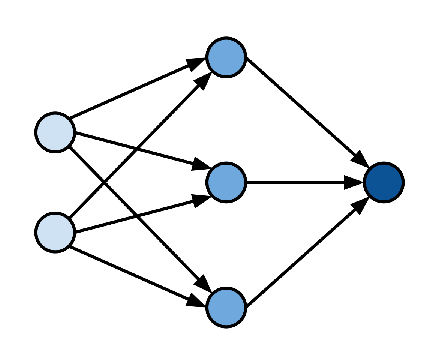
\includegraphics[width=.45\textwidth]{nn.pdf}
	\caption{Neural network with one hidden layer}
	\label{fig:ex}
\end{figure}

\subsection{Algorithms}
Algorithms can be generated by means of the algorithmic package. An exemplary output looks like \autoref{alg:ex}. We refer to the source code of this document or to the algorithmic package documentation for detailed information.


\begin{algorithm}\caption{Automatic Thresholding Algorithm}\label{alg:ex}
	\begin{algorithmic}
	\STATE Init: Initial guess $T$, Tolerance $\epsilon$
	\STATE $dt := 2\epsilon$
	\WHILE {$(dt > \epsilon)$}
		\STATE $G_1 := \begin{Bmatrix} I_{i,j}: I_{i,j} > T \end{Bmatrix}$
		\STATE $G_2 := \begin{Bmatrix} I_{i,j}: I_{i,j} \leq T \end{Bmatrix}$
		\STATE $m_1 :=$ Average value of $G_1$
		\STATE $m_2 :=$ Average value of $G_2$
		\STATE $T' = \frac{(m_1 + m_2)}{2}$
		\STATE $dt = \lvert T - T' \rvert$
		\STATE $T = T'$
	\ENDWHILE
	\STATE return T
	\end{algorithmic}
\end{algorithm}

\subsection{Tables}
\autoref{tab:ex} shows an example of a table. Adapt the source code of this documents to your needs and check the booktabs package documentation, which is used in the present template.

\begin{table}
	\centering
	\caption{Comparison of the segmentation performance}
	\label{tab:ex}
	\begin{tabular}{l l c c c}
		\toprule

		%\multicolumn{2}{l}{\textbf{Class}  stat. Method} \\
		\textbf{Class} & \textbf{stat. Method} \hspace{0.6cm} & \multicolumn{3}{l}{\textbf{Segmentation accuracy in \% $\pm \text{ 1 } \sigma$}}\\
		\cmidrule{1-5}
		Background &  & correct & $\rightarrow$ DNA strand \\ 
		\cmidrule{3-5}
			 & PostProcessing(SVM) 	& $ 99.545 \pm 0.081 $ & $ 0.455 \pm 0.081 $ \\
			 & USZ-Method			& $ 99.798 \pm 0.039 $ & $ 0.202 \pm 0.039 $ \\
			 & Cancer Research App	& $ 99.973 \pm 0.013 $ & $ 0.027 \pm 0.013 $ \\

		\cmidrule{1-5}
		DNA strand &  & correct & $\rightarrow$ Background \\ 
		\cmidrule{3-5}
			 & PostProcessing(SVM) 	& $ 96.704 \pm 1.288 $ & $ 3.296 \pm 1.288 $ \\
			 & USZ-Method			& $ 84.795 \pm 1.556 $ & $ 15.204 \pm 1.556 $ \\
			 & Cancer Research App	& $ 95.513 \pm 2.03 $ & $ 4.488 \pm 2.03 $ \\

		\bottomrule
	\end{tabular}
\end{table}


\subsection{Listings}
All listing should be stored in the codesamples subfolder and they are included with \texttt{\textbackslash lstinputlisting[caption=..., float=tbph, label=...]{codesamples/listname}}. The current setting is optimized for C++. Adapt the settings to your needs in formatAndDefs.tex around line $30$. In case you need other keywords (e.g. Cuda stuff) add the keywords to the list of "morekeywords in Line $52$ in the formatAndDefs.tex file. \autoref{list:ex} shows a trivial listing example.

\lstinputlisting[caption=\texttt{int main} example listing, float=tbph, label=list:ex] {codesamples/intmain.cpp}

\subsection{AutoRefs}
Instead of \texttt{\textbackslash ref} we use \texttt{\textbackslash autoref} which generate better looking links, e.g. \autoref{fig:ex}, \autoref{alg:ex}, \autoref{tab:ex} or \autoref{list:ex}. The keywords can be change around line $186$ in formatAndDefs.tex.

\subsection{References}
All references are generated as usual with \texttt{\textbackslash cite}. The only difference is that we generate a back-link from the list of references to the place where you cited the reference. For example you see under the references that I cited \cite{wiki} on this page. In addition all references are links.

\subsection{General formating}
Play around with empty pages between the different chapters in order to ensure that all chapters begin on a right page.




%\newpage
%\mbox{ }
%\thispagestyle{empty}

\section{Conclusions and Outlook}
\label{sec:6}

\vspace{.6cm}
\secttoc
\vspace{.6cm}

\subsection{Conclusions}
Proin venenatis ornare orci, volutpat viverra ante posuere eu. Quisque posuere sem lacus, ultrices ultricies velit. Nam venenatis ultrices libero, ut molestie turpis scelerisque sed. Donec ut tortor elit. Quisque venenatis volutpat massa, lacinia egestas lorem luctus ut. Phasellus sagittis vulputate massa, ac suscipit nibh rutrum at. Cras gravida, lorem nec porta venenatis, est nisi egestas orci, at bibendum risus eros nec erat. Pellentesque gravida, metus vitae faucibus ultrices, urna ante lacinia tellus, in condimentum lorem erat et ipsum. Ut gravida auctor facilisis.

Phasellus mattis, nibh sit amet laoreet pharetra, mi felis hendrerit tellus, vel lobortis velit massa ac tortor. Nam orci risus, dictum non tincidunt ac, iaculis sed augue. In accumsan dictum dui vel feugiat. Nulla nisi ligula, fermentum sed pretium at, viverra id nibh. Vestibulum ante ipsum primis in faucibus orci luctus et ultrices posuere cubilia Curae; In rutrum nulla a dolor pulvinar blandit. Vestibulum ligula elit, interdum ut ornare consectetur, congue id lectus. Cras iaculis odio quis eros condimentum vulputate mattis odio tincidunt. Proin aliquet lacinia dignissim. Donec a pretium magna.

Fusce eu enim felis. Sed et felis nunc, at vehicula dolor. Duis quis arcu vel est pellentesque ornare vel non nisi. Integer varius lorem a ligula commodo vestibulum. Sed malesuada eleifend sollicitudin. Morbi arcu lorem, consequat eget aliquam euismod, malesuada quis libero. Sed aliquam urna in odio luctus ut gravida lacus mattis. Suspendisse malesuada ante nec lectus pellentesque a condimentum nunc facilisis. Mauris eleifend arcu ut sapien vulputate id sollicitudin diam tristique. Nullam ac massa in sem consequat bibendum ut vitae lectus. Morbi ac porttitor turpis. Aliquam erat volutpat.

\subsection{Future Work}
Lorem ipsum dolor sit amet, consectetur adipiscing elit. Integer odio diam, pharetra commodo pulvinar eget, elementum quis velit. Quisque commodo dolor turpis. Sed quam dui, fringilla a lacinia quis, mollis a risus. Integer adipiscing interdum augue vel porttitor. Sed mollis auctor laoreet. Aliquam ligula leo, convallis at iaculis at, viverra ut elit. Proin commodo sem eu ipsum sollicitudin in ultrices sem adipiscing. Sed facilisis, enim a feugiat iaculis, nulla ante suscipit ipsum, eget scelerisque ligula urna id eros. Maecenas imperdiet gravida est eget semper. Phasellus sapien libero, accumsan quis euismod eu, placerat vitae justo. Curabitur non velit nisi, non pretium lacus. Praesent sed imperdiet lectus. Curabitur eleifend fringilla magna non pretium. Duis sed tellus sed nulla dapibus sodales sed vitae est.

Aliquam erat volutpat. Vivamus nisi elit, placerat in vehicula a, ornare in quam. Vestibulum porta ornare euismod. Aliquam eleifend pretium magna, ac ullamcorper est dignissim id. In hac habitasse platea dictumst. Quisque varius lectus et est porta dapibus. Nulla facilisi. Pellentesque libero risus, bibendum ac rutrum in, feugiat sed sapien.




\thispagestyle{empty}

%
% Appendix
%

\appendix
\section{First Appendix}
\label{app:1}

Lorem ipsum dolor sit amet, consectetur adipiscing elit. Integer odio diam, pharetra commodo pulvinar eget, elementum quis velit. Quisque commodo dolor turpis. Sed quam dui, fringilla a lacinia quis, mollis a risus. Integer adipiscing interdum augue vel porttitor. Sed mollis auctor laoreet. Aliquam ligula leo, convallis at iaculis at, viverra ut elit. Proin commodo sem eu ipsum sollicitudin in ultrices sem adipiscing. Sed facilisis, enim a feugiat iaculis, nulla ante suscipit ipsum, eget scelerisque ligula urna id eros. Maecenas imperdiet gravida est eget semper. Phasellus sapien libero, accumsan quis euismod eu, placerat vitae justo. Curabitur non velit nisi, non pretium lacus. Praesent sed imperdiet lectus. Curabitur eleifend fringilla magna non pretium. Duis sed tellus sed nulla dapibus sodales sed vitae est.

Aliquam erat volutpat. Vivamus nisi elit, placerat in vehicula a, ornare in quam. Vestibulum porta ornare euismod. Aliquam eleifend pretium magna, ac ullamcorper est dignissim id. In hac habitasse platea dictumst. Quisque varius lectus et est porta dapibus. Nulla facilisi. Pellentesque libero risus, bibendum ac rutrum in, feugiat sed sapien.





\newpage
\mbox{ }
\thispagestyle{empty}
\newpage


\bibliographystyle{ThesisStyleWithEtAl}
\bibliography{thesis}

\newpage
\thispagestyle{empty}
\mbox{}
\newpage

\listoffigures

\newpage
\thispagestyle{empty}
\mbox{}
\newpage

\lstlistoflistings

\newpage
\thispagestyle{empty}
\mbox{}
\newpage

\listoftables

\newpage
\thispagestyle{empty}


\end{document}
